\section{To eat of the Tree}

\begin{wrapfigure}{rt}{.3\textwidth}
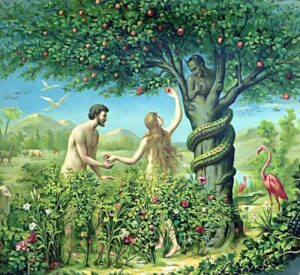
\includegraphics[scale=.4]{TreeOfKnowledge-300x275.jpeg}
\end{wrapfigure}

The archetypal sin is described in the chapter 3 of the Book of Genesis, every sin being a repetition, or an application to a particular situation of this primal error. This episode has been greatly abused, both by critical rationalists and by ``fundamentalists'' who refuse to admit anything beyond the literal understanding. Of course, this episode also has a historical, or better yet sacred historical meaning, as the end of the Golden Age of our aeon and the starting point of the gradual decline that followed, but my main purpose here will be to approach it from a microcosmical perspective, from the point of view of the inner constitution of man and his faculties.

\paragraph{In the image and likeness of God}


Created in the image and likeness of God, man inhabits an intermediate state. He cannot stand on his own, as an independent monad. We will see later what this means.

To be in the image of God is equivalent to saying that man's being is a complete reflection of the being of God. It doesn't mean that a certain part of man is in this Image, but that man as a whole --- this includes his primordial body, illustrated by Christ after the Resurrection, as opposed to the opaque body that is the result of the fall --- is a mirror of the Absolute. Opened towards the infinite, man has the whole within himself, imparted to him through Grace. \textbf{St. Gregory of Nazianz} speaks of this fact: ``Man is a creature that was commanded to become god. The image implies man's destiny in godhood''. The likeness, on the other hand, implies that man is to use the attributes which spring from his being (the image of God) to act according to the divine Order. Just as God sustains, with His uncreated energies, the whole cosmos according to a rigorous law, so man is to act upon the nature he has been given to rule, with his attributes, in conformity with sacred principles, and not to some arbitrary fancy.

\textbf{St. Gregory Palamas}, along with some other philokalic Fathers, says that the fall from the primordial state implied a loss of the likeness with God, while the image, although it was retained and can never be nullified, increasingly obscure and distorted, acquiring more and more a status of a virtuality, no longer fully realized and accessed by fallen humanity. Hence the need for initiation (Baptism) and other sacramental rites that give us the possibility to make the image active once more and, also, to regain the likeness.

The primordial state implied an undifferentiated inner unity in man. Since I intend to write from a microcosmical perspective, the names of ``Adam'' and ``Eve'' will be taken in a special way, as symbols of inner faculties of the human being. The birth of Eve from Adam's rib can be interpreted as the separation of Heaven and Earth, repeated in the microcosm, a first differentiation in the interior constitution of man- remaining, however, unified. In geometrical symbolism, this can be represented by the passing from the circle to the ellipse --- a polarization of the center in two complementaries.\footnote{See Rene Guenon: \textit{Symbols of Sacred Science}, Chapter XXXII.}

Adam, here, is the fiery part, always in contact with Heaven, while Eve is the humid part, in contact with the earth. Adam is passive in respect to Heaven and active in respect to Eve, while Eve is passive towards Adam, but active towards the earth. Generally speaking, primordial man is passive in relation to God, receiving from him the uncreated energies that sustain his being, and he is active in relation to the earth, passing the uncreated energies received from above, to the realm bellow, ordering nature according to divine order --- as above so bellow, on Earth, as it is in Heaven. On the inner plane, the intellect rules the desiring faculty and both act in unity. In other words, primordial man knows God in all things and desires nothing but God and the acting of God's will upon the earth.

Eve's dependency on Adam is underlined in some of the patristic teachings, that she received the command not to eat from the Tree of Knowledge of good and evil indirectly from Adam, who received it directly from God. Adam, being the ruling principle in man, is responsible for the ordering of the being according to the divine laws, while Eve must act in obedience to these laws and pass them forward towards nature.

\paragraph{Knowledge of good and evil}


The tree of knowledge of good and evil is a symbol of dualism, of separation. Here is what \textbf{St. Maxim the Confessor} has to say regarding it:

\begin{quotex}
Since man came into being made with an intellectual spiritual soul and a body equipped with senses, after a first meaning, the Tree of Life is the intellect, the seat of wisdom, and the Tree of Knowledge of good and evil is the bodily sense, where, clearly, the irrational movement has its beginning. Both trees give the ability to discern between various things. ... The intellect has the ability to discern between the spiritual and the sensual, the eternal and the ephemeral ... while feeling discerns between physical pleasure and pain. (Quoted and translated from the Romanian Philokalia, Maxim's answers to Thalassios).
\end{quotex}


A Romanian theologian, \textbf{Dumitru Staniloae}, adds that the fall implied a break between the various faculties, mankind concentrating much of its efforts on the lower, irrational ones, oscillating between two equally illusory extremes, that fuel each other --- those of pleasure and pain:

\begin{quotex}
Man's inclination towards the sensory stirs his pleasure for it, turning all his energy away from the spirit only to what comes under the senses ... he does not give away pleasure as the cause of pain , but turns himself to it in order to get rid of the pain, wrapping himself into an ever thickening vicious circle. (Translated from Romanian, from a book called ``The asceticism and mysticism of the Orthodox Church'').
\end{quotex}


The two authors give good and evil a horizontal meaning, as two opposite (but in truth complementary) aspects of an illusory horizontal line. I believe, however, that it could be also interpreted in a relatively vertical way. Good being that which leads back towards unity (or at least keeps one closer to it), while evil is that which deepens the fall, leading further into fragmentation and dissolution. However, neither one can exist without the other. For example: gluttony is evil, fasting good. Gluttony thickens the body which then leads the soul into a stupor, making the access towards the pneumatic faculties impossible. Fasting purifies the body and makes it a suitable support for the spirit. However, there would be no need for fasting were man's body pure, just as medicine is unthinkable for a healthy person. Thus, ``good'', in this case, is only relative, being actually a necessary evil (from the point of view of matter) meant to repair a greater evil. Primordial man is beyond good and evil, because he knows the true Good (which is plenitude). Fallen man knows good \textbf{AND} evil, and can never disconnect them from one-another so the only option available is to transcend them. I think such an interpretation is also echoed in the parable of the prodigal son.

Again, in the words of St Maxim, ``the saint extinguishes all opposition within himself''. Here is the real doctrine of going beyond good and evil. It is not, as Nietzsche believed it --- the destruction of all standards in order to replace them with some arbitrary ones, conceived by a promethean will --- but the ultimate conformity with spiritual Reality.

\paragraph{The stages of sin}


Looking now at the actual occurrence of the primal sin, we see multiple stages of it. The inception comes through the subtle approach of the devil --- the centrifugal pseudo-principle of inferior chaos, that opposes divine order and seeks to pull creation into the pulverizing illusion of the outer darkness. ``And he said unto the woman, Yea, hath God said, Ye shall not eat of every tree of the garden?'' (Gen. 3.1). He approaches Eve, as the principle in man directly in contact with the earth. The fact that he managed to approach her may also suggest a temporarily negligence on account of the intellect (Adam). In this first stage, the demonic force only attempts to initiate a dialogue with the desiring part of man. Since a dialogue is a series of emissions and receptions, both partners sending and \textbf{receiving} ideas from each other, this would imply that Eve will have to enter into relation with these lower forces and receive some influence from them. The fact that she accepts a dialogue immediately makes her temporarily passive towards the inferior regions, leading to a direct suggestion:

\begin{quotex}
And the serpent said unto the woman, Ye shall not surely die: For God doth know that in the day ye eat thereof, then your eyes shall be opened, and ye shall be as gods, knowing good and evil.
\end{quotex}


This is the primal temptation: the illusion of becoming independent from God, of pursuing a self-sufficient existence, completely closed and uninfluenced by anything above.

\begin{quotex}
And when the woman saw that the tree was good for food, and that it was pleasant to the eyes.
\end{quotex}


That is, Eve only considered the fruits according to their most outer appearance, in a sensual manner, severed from their deeper significance, not making any use of the ordering faculty of the intellect and a tree to be desired to make one wise, i.e., a wisdom understood only according to a limited and exterior point of view

\begin{quotex}
she took of the fruit thereof, and did eat, and gave also unto her husband with her; and he did eat.
\end{quotex}


Eve, the desiring and receptive faculty, by eating of the fruit, became active towards Adam, the intellectual and ordering principle and passive towards the earth and the lower regions. Adam, instead of correcting this error he participated by approving the indulgences of desire, becoming himself active in relation to God and passive towards Eve. Adam's mistake is graver than Eve's, since Adam is the intellect who has supreme responsibility for the maintaining of the divine order in creation. It is only after he ate that ``their (physical) eyes opened''. The message is that, even though the sensual part begins to rebel, all is not lost and may be corrected by the rational part who is responsible to keep it in check; but if reason also participates in the act, the point of no return has been passed. This is why the unseen warfare is primarily concerned with the battle over the mind. A parallel of the episode in Genesis can also be found in \emph{Proverbs}, chapter 7:

\begin{quotex}
My husband is not at home, he has gone on a long journey
\end{quotex}


This means that the rational faculty left the center --- the spirit --- and concerns itself with the circumference, the external world of appearance; his hands are filled with money meaning that it is unable to act --- filled hands --- having concerned itself with multiplicity, away from the primordial unity \paragraph{God's judgement}


God's judgement upon fallen man is not to be regarded as some legalistic, external punishment. In Genesis, God appears sometimes to directly sentence the fallen couple ``I will greatly multiply thy sorrow and thy conception; in sorrow thou shalt bring forth children'' while other times He simply observes the changing of state that man and nature undergo: ``cursed the ground for thy sake; in sorrow shalt thou eat of it all the days of thy life''.

This should be understood in the light that Divine Justice means to put each and all according to their rightful place and status. When man acts according to illusory purposes, fragmenting the essential unity of creation, he operates a similar fragmentation within himself (because of the analogy that always exists between macrocosm and microcosm), suffering an ontological degradation, creating a sympathy bond with an inferior level of existence. God sends one to the level that one, of one's own accord, has chosen. Thus, the fact that man became subject to death/demons/disease/decay, is not some external, arbitrary punishment on God's part, but the consequence of man having attached himself to things pertaining to a level of existence where it is possible to be affected by hostile forces. If I make money, for example, the supreme goal of my life, I become attached to them, the standard according to which I measure myself. Since this ``standard'' is on a level of existence of perpetual becoming and fluctuations I will share its ups and downs, opening myself up to insecurity, fears, hopes, depression etc. If God is also said to condemn us is because, being the supreme Subject, He cannot be an impersonal, passive observer in respect to any process, but is the primary Mover of all things.

There is one last issue to consider before drawing conclusions. Namely the notion of ``original sin''. It must be said that in the Eastern Church this notion was never accepted as it is proposed in the West. What I mean is that, here, human beings do not ``inherit'' Adam's guilt. It is just that the degradation of the macrocosm and the inherited traits from one's ancestors make it harder, for descendants born in later times, to understand Reality and access higher faculties without direct divine Revelation and certain Divine-established rites, meant to reawaken the Image in man. This means that, for example, a person born in the Iron Age --- the whole period which we call ``historical'' --- does not enter the world with a ``stained'' soul. It is just that the cosmic conditions in such a time and the physical and psychic elements passed to him from his direct ancestors make him susceptible to develop his inferior possibilities (since all external conditions are right for such), while the Truth is very difficult to be discovered without external aid. He may attain the highest summit, but he has to fight his way to it; but first he must become conscious of his higher calling, which may prove the more difficult. Better put, he is in a small part actually human, while the largest part of his humanity lies dormant, in a state of virtuality. Of course, each period presents some compensations.

\paragraph{Conclusions}


After all this, we can conclude that sin is a revolt of the part against the whole, the considering of objects (as well as other beings and persons) independent from their inner purpose, their inner reason for existence. It also implies a misuse of the possibilities of the human being, the employing of human faculties, meant to be directed towards the Infinite, in pursuing illusory, finite objectives, apart or contrary to cosmic order. Using a neoplatonic template, adopted very successfully by Dionysius the Areopagite, the hierarchy of being depends on each given level or degree of existence to be correctly polarized (as showed above)- passive towards the superior level and active towards the inferior. When any being or faculty attempts a schism towards its superiors, the structure collapses, and the being disintegrates, along with all its pretenses.

Sin begins with a diabolical suggestion. When the rational subject is not watchful, his lower nature may enter into dialogue with the suggestion, flirt with it, and slowly come under its influence, especially through the imaginative faculty, at which, we should look at in a different article. After a while, the desiring part will break with the rule of reason and try to pursue the suggestion. If reason does not, through the will, act with firmness, it will begin, slowly, to be dragged into the mire of the irrational soul. The consent of the mind results in the immersion of the entire being in the act.

By consenting to the act, man operates an inversion of polarities within himself. He becomes active in relation to the Sky --- meaning that he deliberately refuses the divine energies that sustain his being --- and passive in relation to the earth --- he is dragged down by inferior influences. As a result of this, man's inner constitution becomes chaotic, disordered, his heart is a battle ground where the unseen warfare takes place. Externally, he becomes an agent of disorder in nature and his surroundings. Just as the saint, or the superior man in general, who is a medium through which divine energies are manifested, has an ordering and stabilizing effect upon nature and other persons, so the inferior man, ruled by passions, is a tool for infernal energies, having a destructive effect on the surroundings- just consider how it feels when sharing a space with a calm, wise and kind person as opposed to someone who is extremely furious, frustrated, agitated or hateful.

Such is the archetypal sin, which is repeated according to circumstance in all particular situations. The inversion of polarities is the way it is effected. Since man is an intermediate creature, he cannot stand on his own, hanging in midair, in complete neutrality and indifference. He either consciously subjects himself to the influence of Heaven --- which keeps him in his place as sovereign and lord of nature, as well as open to the Infinite, to the possibility of godhood- or he rejects Heaven and is dragged down by the gravitational pull of Hell. If man rejects what he has in common with the angels, he loses even what differentiates him from animals, going even lower than them. History --- especially sacred history --- proves this.

On a more particular scale, it can account for the gradual degeneration that has occurred in western mentality, beginning from the time of the Renaissance, when western man became indifferent towards higher realities, going through the active opposition to them by militant rationalism and immediately falling towards an increasing irrationalism, down to the very bottom of sub-human possibilities; having reached Jung's notion of the collective unconscious and the quasi-religious attitude towards it, it is hard to imagine that man's conception of his being and his faculties of knowledge can fall any lower. But it is a logical conclusion after the part (reason) attempted to become independent of the whole (the intellect, or the heart as a symbol for the spirit). The principle of polarities outlined above explains very well why rationalists are very sharp in employing reason against the higher realities, but are absolutely powerless in the face of the most degrading irrationalities. Reason, refusing the illumination of the higher, cannot but receive the darkness of the lower.

I will continue, in the future, to address through a more particular approach the notion of ``unseen warfare''.

\paragraph{Updated 21 Feb 2021} This was Holy Fool's last post. He had previously been an enthusiastic supporter and active commenter. He suddenly left without explanation, secretly removing all his posts on the way out. He allowed me to keep this one, provided it is published anonymously.

So much for the warrior ethos of loyalty and integrity.

\flrightit{Posted on 2013-02-21 by Holy Fool}

\begin{center}* * *\end{center}

\begin{footnotesize}
\begin{sffamily}
\texttt{vivianiprimo on 2020-02-23 at 09:35 said:}

Amazing piece of writing, thank you so much!

\hfill

\texttt{Lee on 2020-03-23 at 02:59 said:}

Ok, this is helpful. Passive in relation to the Divine, active in relation to creation.

\end{sffamily}
\end{footnotesize}

